\chapter{Public services in Smart Cities}
\label{intro} 



\section{Introduction}
\label{sec:1}
\subsection{Motivation}
Smart cities are a possible and likely future. Smart mobility is a big part of it and automated and controlled emergency vehicles will be a part of it. 
\subsection{Emergency vehicles and automation}
When a cars crashes or has another emergency like an unconscious driver, it can send an emergency call to the server. The server then tells the emergency vehicles to move to the accident site. The emergency vehicles can then drive to a available hospital. This will all happen automatically.

\section{Concept}
\label{sec:3}
Emergency vehicles have to act fast and efficiently, in case of an emergency. That's why it is important to know where the emergency vehicles are and if they are available.
\newline
The communication with the server is based on topics. Each vehicle has its own topic for communication (for example "/hshl/polices/p1" where "p1" is the vehicle id of a police car).  The created / available vehicle information is send to the server. If an emergency happens, the server requests vehicles to move to the location of the emergency. The program checks if the requested vehicles are available. If they are, they are send to the place of operation. Once the vehicles arrive, the server is notified of the arrival. The Server is also notified when the vehicles eventually return. 
\newline
The emergency vehicles also need a certain amount of people to operate. The police-car needs two officers, the ambulance a driver and a doctor and the fire engine need at least 6 firefighters.
\newline
\subsection{Requirements}
\begin{center}
\begin{tabular}{ c c }
  & Functional Requirements \\
   \hline\hline
 F1 & The vehicles has to show the amount of people inside. \\ 
 F2 & The vehicles has to show the individual people inside. \\  
 F3 & The vehicles has to show its current GPS coordinates. \\
 F4 & People have to be able to enter and leave the vehicles. \\
 F5 & Information of available vehicles has to be send to the \\
 F5 & server whenever there is a change in the amount. \\
 F6 & Vehicles have to be able to receive information / tasks from the server. \\
 F7 & Vehicles have to confirm the received information. \\
 F8 & Vehicles have to confirm the arrival at the place of operation to the server. \\
 F9 & Vehicles have to send information about the people inside \\
 F9 & to the server when they leave the place of operation.\\
 \\
  & Non-Functional Requirements \\
   \hline\hline
 NF1 & The confirmation of the revived information should not take longer than 5 seconds.\\
 NF2 & The confirmation of the arrival at at the place of operation \\
 NF2 & should not take longer than 5 seconds.\\
 NF3 & The ambulance must have at least 2 people to operate.\\
 NF4 & The ambulance can not hold more than 6 people at once.\\
 NF5 & The police-car must have at least 2 people to operate.\\
 NF6 & The police-car can not hold more than 5 people at once.\\
 NF7 & The firefighting vehicle must have at least 2 people to operate.\\
 NF8 & The firefighting vehicle can not hold more than 9 people at once.\\
 NF9 & The firefighting vehicle should always operate with at least 6 firefighters.\\
 NF10 & The software has to be implemented with python.
\end{tabular}
\end{center}
\newpage
\subsection{Use Case}
\begin{figure}[!h]
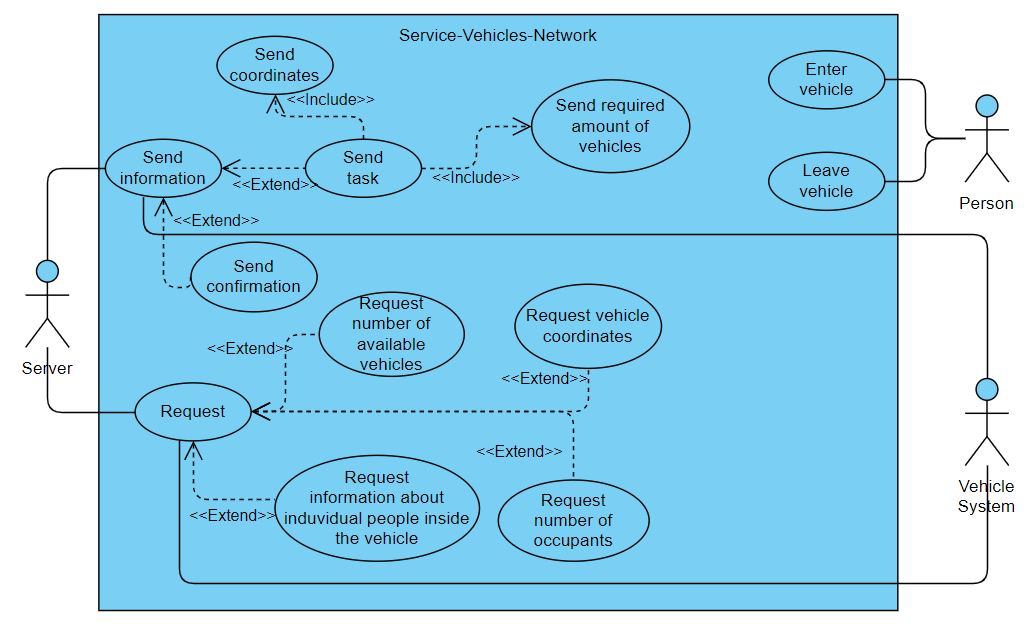
\includegraphics[scale=0.5]{images/Heiber/b0.JPG}
\caption[caption]{Use case}
\end{figure}

\section{Implementation}
\label{sec:4}
This section describes the implementation of the program. Here only one of the three implementations for the vehicles is shown, since they are mostly the same.
\subsection{Main Program}
The main program manages the vehicles and the communication with the server. The timing simulation is implemented in the "test" program.
\newline
\newline
First the program imports necessary libraries:
\begin{figure}[!h]
\center
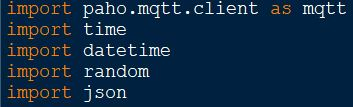
\includegraphics[scale=0.6]{images/Heiber/a0.JPG}
\caption[caption]{Used libraries}
\end{figure}
\newline
MQTT or Message Queuing Telemetry Transport is an open OASIS and ISO standard (ISO/IEC 20922) lightweight, publish-subscribe network protocol that transports messages between devices.
\newline
The libraries "time" and "datetime" are used to get the local time and date.
\newline
The library "random" is used to generate a random number. In the case of the implementation it will help randomizing the coordinates of the vehicles and assigning random names to the vehicles.
\newline
The library "json" is for en- and decoding json files for easier communication between the server and the main program. Its used to save information and is easy to access and use.
\begin{figure}[!h]
\center
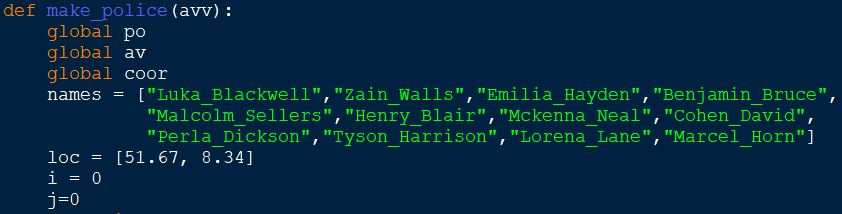
\includegraphics[scale=0.6]{images/Heiber/a1.JPG}
\caption[caption]{Method "make\_police" 1/5}
\end{figure}
\newline
In the method "make\_police" the vehicles are created.
The "global" in front of the variables are used to save the variables not just in the method, but also in the main program. The list of names is used to fill the positions of the vehicle. In this case it would be two officers. The "loc" variable stores the coordinates of the city Lippstadt in Germany. 
\begin{figure}[!h]
\center
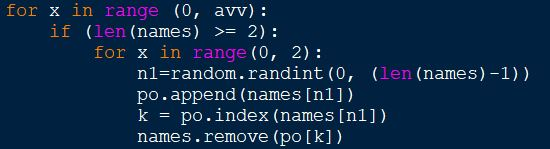
\includegraphics[scale=0.6]{images/Heiber/a2.JPG}
\caption[caption]{Method "make\_police" 2/5}
\end{figure}
\newline
The fist for loop is responsible for the creation of multiple vehicles. It runs as many times as the number specified in the variable "avv". The if statement makes sure to only create a police car, if there are enough "officers" available. The second for loop is for actually assigning the officers. Here a random "officer" is taken from the names list and added to the "po" list. The name is also removed from the names list. This prevents it from being used twice. This fulfils the requirement NF5.
\newpage
\begin{figure}[!h]
\center
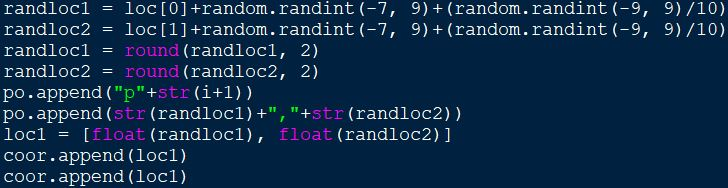
\includegraphics[scale=0.6]{images/Heiber/a3.JPG}
\caption[caption]{Method "make\_police" 3/5}
\end{figure}

Here the starting locations of the vehicles are randomized based on the locations of Lippstadt (variable "loc"). The coordinates are than stored in the "po" list. The id of the vehicle is also added to the "po" list.
\begin{figure}[!h]
\center
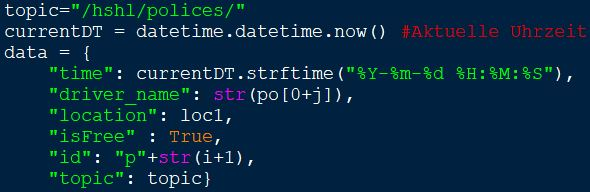
\includegraphics[scale=0.6]{images/Heiber/a4.JPG}
\caption[caption]{Method "make\_police" 4/5}
\end{figure}
\newline
At this section we assign a topic to which the data from the next step will be send. The current date and time is saved and a json data pack is created. It contains the time, date, name of the driver (one of the officers), the location of the vehicle, the id and the topic.
\begin{figure}[!h]
\center
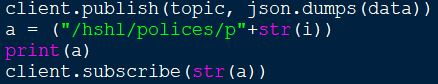
\includegraphics[scale=0.6]{images/Heiber/a5.JPG}
\caption[caption]{Method "make\_police" 5/5}
\end{figure}
\newpage
In the last part of the method the program subscribes to the topic of the vehicle (vehicle id) and shows the topic in the console.
\begin{figure}[!h]
\center
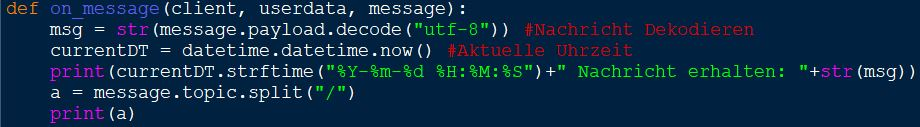
\includegraphics[scale=0.6]{images/Heiber/a6.JPG}
\caption[caption]{Method "on\_message" 1/2}
\end{figure}
\newline
The method "on\_message" is called when a message is send to one of the subscribed topics. It displays  the date and time of arrival, the massage itself and the topic of the message.
\begin{figure}[!h]
\center
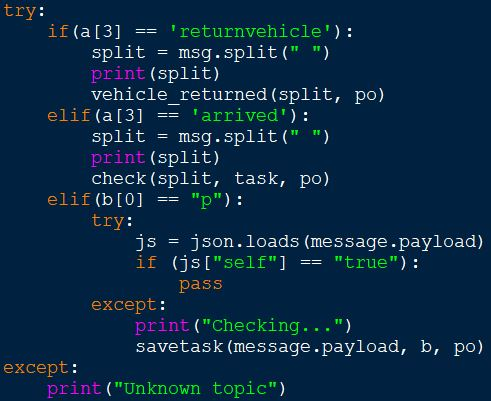
\includegraphics[scale=0.6]{images/Heiber/a7.JPG}
\caption[caption]{Method "on\_message" 2/2}
\end{figure}
\newline
Then it decides which method should be called next. If the message was send from the program itself, the message includes a "self" variable. This way, only messages from itself will be ignored. This fulfils the requirement F6
\begin{figure}[!h]
\center
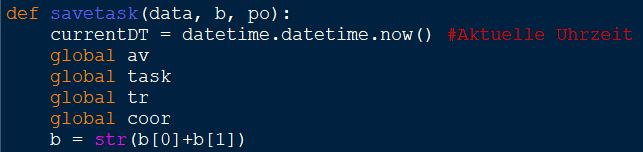
\includegraphics[scale=0.6]{images/Heiber/a8.JPG}
\caption[caption]{Method "savetask" 1/5}
\end{figure}
\newline
The method "savetask" is called when a vehicle is requested from the server. Here the variable "b" contains the vehicle id, the variable "av" contains the current amount of available vehicles, "coor" stores the current coordinates of the vehicle as well as the coordinates of the place of operation. The variable "tr" is used to reduce the possibility to influence the program from wrong messages. In the variable "task" the request of the server is stored until the task has been done. Although it is only saved when the task has been accepted.
\begin{figure}[!h]
\center
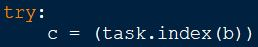
\includegraphics[scale=0.6]{images/Heiber/a9.JPG}
\caption[caption]{Method "savetask" 2/5}
\end{figure}
\newline
These two lines of code check if a vehicle has a task already. If so, the request of the server will be denied.
\begin{figure}[!h]
\center
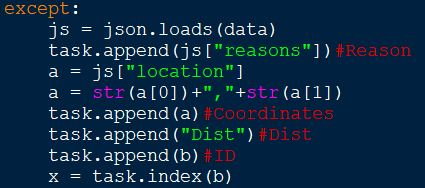
\includegraphics[scale=0.6]{images/Heiber/a10.JPG}
\caption[caption]{Method "savetask" 3/5}
\end{figure}
\newline
If the vehicle is still available, the task is saved.
\begin{figure}[!h]
\center
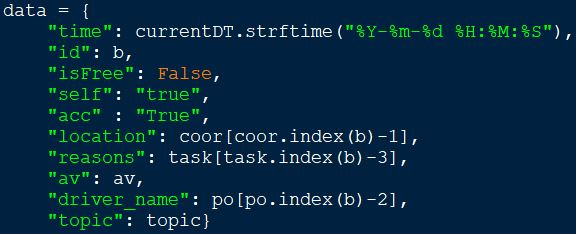
\includegraphics[scale=0.6]{images/Heiber/a11.JPG}
\caption[caption]{Method "savetask" 4/5}
\end{figure}
\newline
Then a json data pack is created. All necessary information is saved in it. This fulfils the requirements F3 and F5.
\newpage
\begin{figure}[!h]
\center
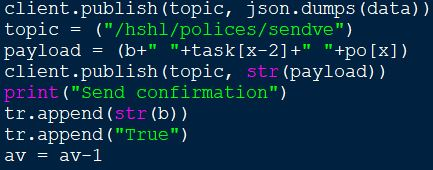
\includegraphics[scale=0.6]{images/Heiber/a12.JPG}
\caption[caption]{Method "savetask" 5/5}
\end{figure}
The method send a short message to the "Test" program and a message containing the data pack to the server, accepting the task.
\begin{figure}[!h]
\center
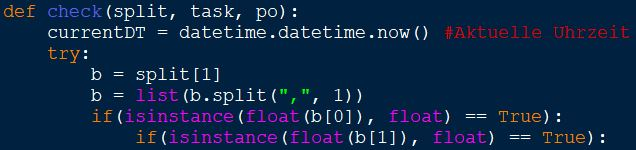
\includegraphics[scale=0.6]{images/Heiber/a13.JPG}
\caption[caption]{Method "check"}
\end{figure}
\newline
The methods "check" and "vehicle\_returned" check if the coordinates of the received message from the "test" program are coordinates and not a string or else. If so, they send the new coordinates to the server. The method "vehicle\_returned" also tells the server, that the vehicle is available again and removes the old task. This fulfils the requirement F8.
\subsection{Secondary Program}
The "test" program was written to simulate a time difference between departure time and arrival time of the vehicles. It does so twice, once for the travel to the place of operation and the return journey.
\begin{figure}[!h]
\center
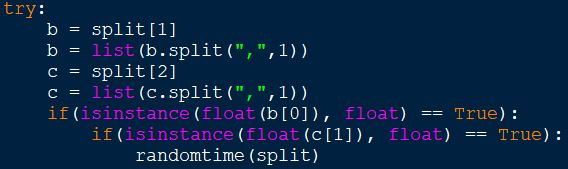
\includegraphics[scale=0.6]{images/Heiber/a14.JPG}
\caption[caption]{Main of "test" program}
\end{figure}
\newline
It too fist checks the coordinates, then calls the method "randomtime".
\begin{figure}[!h]
\center
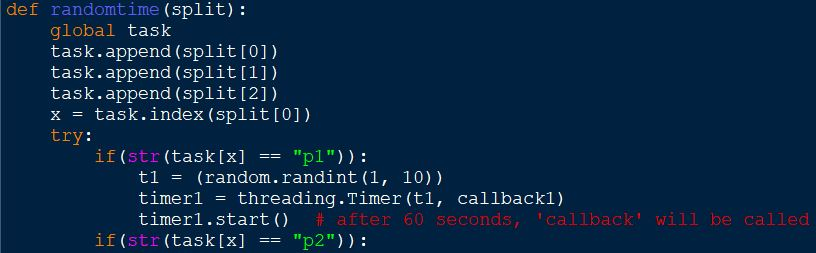
\includegraphics[scale=0.6]{images/Heiber/a15.JPG}
\caption[caption]{Method "randomtime"}
\end{figure}
\newline
The method "randomtime" saves the coordinates and start a timer using threads. If the timer expires, the next method is called. This happens between the run time. This means, the program stops what its doing and first executes the called method, then it resumes the previous execution. At the last method, the task is deleted.
\newline

\section{Conclusion}
\label{sec:5}
Not all of the requirements were implemented since many were deemed unnecessary and to improve performance of the main server. These include the strict observation of personal in the vehicles (F2) and the confirmation of the requests (F7). Since personal are no longer tracked, the amount of people inside a vehicle is solely dependent on the personal, so checking for the maximal amount of people has become unnecessary as well (F9, NF4, NF6, NF 8).
\newline
Sadly i had to rewrite the program once and hand to make major changes with the second version. This was because of the late start of communication between members of the project and the change in communication between the server and the program from a json based communication to a string based communication and then back to json. I think it would be better to work together from the beginning. This way anyone in the project can decide on one form of communication and how to communicate in general.

\newpage
\bibliographystyle{IEEEtran}
\bibliography{./chapter.bib}
